%%%%%%%%%%%%%%%%%%%%%%%%%%%%%%%%%%%%%%%%%%%%%%%%%%%%%%%%%%%%%%%%%%%%%%%%%%%%%%%%%%%%%%%%%%%%%%%%%%%%%%%%%%%%
%%%%%%%%%%%%%%%%%%%%%%%%%%%%%%%%%%%%%     TIPO DE DOCUMENTO      %%%%%%%%%%%%%%%%%%%%%%%%%%%%%%%%%%%%%%%%%%%
%%%%%%%%%%%%%%%%%%%%%%%%%%%%%%%%%%%%%%%%%%%%%%%%%%%%%%%%%%%%%%%%%%%%%%%%%%%%%%%%%%%%%%%%%%%%%%%%%%%%%%%%%%%%

\documentclass[12pt,a4paper,openright]{article}

%%%%%%%%%%%%%%%%%%%%%%%%%%%%%%%%%%%%%%%%%%%%%%%%%%%%%%%%%%%%%%%%%%%%%%%%%%%%%%%%%%%%%%%%%%%%%%%%%%%%%%%%%%%%
%%%%%%%%%%%%%%%%%%%%%%%%%%%%%%%%%%%%%     PAQUETES A CARGAR      %%%%%%%%%%%%%%%%%%%%%%%%%%%%%%%%%%%%%%%%%%%
%%%%%%%%%%%%%%%%%%%%%%%%%%%%%%%%%%%%%%%%%%%%%%%%%%%%%%%%%%%%%%%%%%%%%%%%%%%%%%%%%%%%%%%%%%%%%%%%%%%%%%%%%%%%

\usepackage[left=3cm,top=3.25cm,right=3cm,footnotesep=1cm]{geometry}
\usepackage{graphicx}
\usepackage{wrapfig}
\usepackage[spanish]{babel}
\usepackage[utf8]{inputenc}
\usepackage{amsmath}
\usepackage[usenames,dvipsnames]{xcolor}
\usepackage{enumerate}
\usepackage{ragged2e}
\usepackage{float}
\usepackage{appendix}
\usepackage{natbib}
\usepackage{adjustbox}
\usepackage{cite}
\usepackage{relsize}
\usepackage{bbding}
\usepackage{xcolor}
\usepackage{pifont}
\usepackage{hyperref}
\hypersetup{
    colorlinks=true,
    linkcolor=blue,
    filecolor=magenta,      
    urlcolor=blue,
    }

\usepackage{wasysym}
\usepackage{amssymb}
\usepackage{pdfpages}
\usepackage{xcolor}




%%%%%%%%%%%%%%%%%%%%%%%%%%%%%%%%%%%%%%%%%%%%%%%%%%%%%%%%%%%%%%%%%%%%%%%%%%%%%%%%%%%%%%%%%%%%%%%%%%%%%%%%%%%%
%%%%%%%%%%%%%%%%%%%%%%%%%%%%%%%%%%%     OPCIONES DE DOCUMENTO      %%%%%%%%%%%%%%%%%%%%%%%%%%%%%%%%%%%%%%%%%
%%%%%%%%%%%%%%%%%%%%%%%%%%%%%%%%%%%%%%%%%%%%%%%%%%%%%%%%%%%%%%%%%%%%%%%%%%%%%%%%%%%%%%%%%%%%%%%%%%%%%%%%%%%%

\renewcommand{\baselinestretch}{1.25}

%%%%%%%%%%%%%%%%%%%%%%%%%%%%%%%%%%%%%%%%%%%%%%%%%%%%%%%%%%%%%%%%%%%%%%%%%%%%%%%%%%%%%%%%%%%%%%%%%%%%%%%%%%%%
%%%%%%%%%%%%%%%%%%%%%%%%%%%%%%%%%%%%%%%%%%     INICIO      %%%%%%%%%%%%%%%%%%%%%%%%%%%%%%%%%%%%%%%%%%%%%%%%%
%%%%%%%%%%%%%%%%%%%%%%%%%%%%%%%%%%%%%%%%%%%%%%%%%%%%%%%%%%%%%%%%%%%%%%%%%%%%%%%%%%%%%%%%%%%%%%%%%%%%%%%%%%%%

\begin{document}

%%%%%%%%%%%%%%%%%%%%%%%%%%%%%%%%%%%%%%%%%%%%%%%%%%%%%%%%%%%%%%%%%%%%%%%%%%%%%%%%%%%%%%%%%%%%%%%%%%%%%%%%%%%%
%%%%%%%%%%%%%%%%%%%%%%%%%%%%%%%%%%%%%%%%     PORTADA No.1    %%%%%%%%%%%%%%%%%%%%%%%%%%%%%%%%%%%%%%%%%%%%%%%
%%%%%%%%%%%%%%%%%%%%%%%%%%%%%%%%%%%%%%%%%%%%%%%%%%%%%%%%%%%%%%%%%%%%%%%%%%%%%%%%%%%%%%%%%%%%%%%%%%%%%%%%%%%%

\begin{center}
\vspace{-0.5cm}
{\Large\textsc{Universidad Nacional Autónoma de Honduras}}
\vspace{0.5cm}

\begin{center}
  
\includegraphics[width=2cm]{unah}
\end{center}
\vspace{1cm}

{\large
\textsc{Facultad de Ciencias}\\
\textsc{Carrera de Física}\\
\vspace{0.45cm}
\textsc{Maestría en Física}\\
\vspace{0.75cm}
\textsc{T\'opicos de F\'isica Computacional II}\\
}

\normalsize\textsc{Startup Company/Data Analysis Project }
\vspace{1.15cm}

{\large\textsc{Ellis Moises Reyes\\Miguel Angel Serrano}}
\vspace{5cm}




{\large\textsc{Tegucigalpa, Honduras 20 de Agosto, 2021}}

\end{center}


\newpage

%%%%%%%%%%%%%%%%%%%%%%%%%%%%%%%%%%%%%%%%%%%%%%%%%%%%%%%%%%%%%%%%%%%%%%%%%%%%%%%%%%%%%%%%%%%%%%%%%%%%%%%%%%%%
%%%%%%%%%%%%%%%%%%%%%%     INICIO DEL CONTENIDO PRINCIPAL DEL DOCUMENTO     %%%%%%%%%%%%%%%%%%%%%%%%%%%%%%%%
%%%%%%%%%%%%%%%%%%%%%%%%%%%%%%%%%%%%%%%%%%%%%%%%%%%%%%%%%%%%%%%%%%%%%%%%%%%%%%%%%%%%%%%%%%%%%%%%%%%%%%%%%%%%


%%%%%%%%%%%%%%%%%%%%%%%%%%%%%%%%%%%%%%%%%%%%%%%%%%%%%%%%%%%%%%%%%%%%%%%%%%%%%%%%%%%%%%%%%%%%%%%%%%%%%%%%%%%%
%%%%%%%%%%%%%%%%%%%%%%%%%%%%%%%%%%%%%%     ÍNDICE DE CONTENIDOS    %%%%%%%%%%%%%%%%%%%%%%%%%%%%%%%%%%%%%%%%%
%%%%%%%%%%%%%%%%%%%%%%%%%%%%%%%%%%%%%%%%%%%%%%%%%%%%%%%%%%%%%%%%%%%%%%%%%%%%%%%%%%%%%%%%%%%%%%%%%%%%%%%%%%%%

\tableofcontents % indice de contenidos


\newpage

%%%%%%%%%%%%%%%%%%%%%%%%%%%%%%%%%%%%%%%%%%%%%%%%%%%%%%%%%%%%%%%%%%%%%%%%%%%%%%%%%%%%%%%%%%%%%%%%%%%%%%%%%%%%
%%%%%%%%%%%%%%%%%%%%%%%%%%%%%%%%%%%     INTRODUCCION  %%%%%%%%%%%%%%%%%%%%%%%%%%%%%%%%%%%%%%%
%%%%%%%%%%%%%%%%%%%%%%%%%%%%%%%%%%%%%%%%%%%%%%%%%%%%%%%%%%%%%%%%%%%%%%%%%%%%%%%%%%%%%%%%%%%%%%%%%%%%%%%%%%%%

\section{Introducci\'on}

En este documento se describe el proceso de análisis de datos, herramientas que pueden usarse en el desarrollo de un proyecto para mantener la reproducibilidad, un desglose de como usar los recursos para que el proyecto sea realizado en la nube y finalmente una comparación en los costos de estos servicios por parte de diferentes proveedores de PaaS.

%%%%%%%%%%%%%%%%%%%%%%%%%%%%%%%%%%%%%%%%%%%%%%%%%%%%%%%%%%%%%%%%%%%%%%%%%%%%%%%%%%%%%%%%%%%%%%%%%%%%%%%%%%%%
%%%%%%%%%%%%%%%%%%%%%%%%%%%%%%%%%%%     PLANTEAMIENTO DEL PROBLEMA %%%%%%%%%%%%%%%%%%%%%%%%%%%%%%%%%%%%%%%
%%%%%%%%%%%%%%%%%%%%%%%%%%%%%%%%%%%%%%%%%%%%%%%%%%%%%%%%%%%%%%%%%%%%%%%%%%%%%%%%%%%%%%%%%%%%%%%%%%%%%%%%%%%%

\section{Planteamiento del Problema}

Actualmente se dice que los datos son el nuevo "petroleo" o "electricidad". Nos encontramos en la era de los datos, por lo tanto se estan usando en todos los campos, banca, universidades, marketing, econom\'ia, finanzas, pol\'itica, ciencia, gesti\'on de riesgos, log\'istica y muchos m\'as . Actualmente se espera que en los proximos años la demanda de DAAS o servicios de an\'alisis de datos siga en aumento.

%%%%%%%%%%%%%%%%%%%%%%%%%%%%%%%%%%%%%%%%%%%%%%%%%%%%%%%%%%%%%%%%%%%%%%%%%%%%%%%%%%%%%%%%%%%%%%%%%%%%%%%%%%%%
%%%%%%%%%%%%%%%%%%%%%%%%%%%%%%%%%%%%%%%%%%%     JUSTIFICACIÓN   %%%%%%%%%%%%%%%%%%%%%%%%%%%%%%%%%%%%%%%%%%%%
%%%%%%%%%%%%%%%%%%%%%%%%%%%%%%%%%%%%%%%%%%%%%%%%%%%%%%%%%%%%%%%%%%%%%%%%%%%%%%%%%%%%%%%%%%%%%%%%%%%%%%%%%%%%


\section{Justificación}


Nuestra startup busca entrar en un mercado con mucha demanda, que seguira en aumento. Actualmente las empresas mas grandes en el rubro ocupan ayuda de terceros en la limpieza y an\'lisis de los datos, ya que son las partes del proceso de an\'alisis de datos mas demandantes en tiempo.



%%%%%%%%%%%%%%%%%%%%%%%%%%%%%%%%%%%%%%%%%%%%%%%%%%%%%%%%%%%%%%%%%%%%%%%%%%%%%%%%%%%%%%%%%%%%%%%%%%%%%%%%%%%%
%%%%%%%%%%%%%%%%%%%%%%%%%%%%%%%%%%%%%%%%%%%   OBJETIVOS   %%%%%%%%%%%%%%%%%%%%%%%%%%%%%%%%%%%%%%%%%%%%%%%%%
%%%%%%%%%%%%%%%%%%%%%%%%%%%%%%%%%%%%%%%%%%%%%%%%%%%%%%%%%%%%%%%%%%%%%%%%%%%%%%%%%%%%%%%%%%%%%%%%%%%%%%%%%%%%





\section{Objetivos}
\subsection{Objetivo General}
Realizar la propuesta de un proyecto que consiste en una empreza que se encargara de todo el proceso de an\'alisis de datos para cualquier usuarios con cualquier tipo de necesidades.

\subsection{Objetivos espec\'ficos}
\begin{itemize}
    \item Como analistas de datos nuestro objetivo es seguir el proceso de an\'alisis para recolectar, organizar y transformar datos. Para llegar a conclusiones basadas en datos que puedan ayudar a una organizaci\'on, universidad, empresa, compañ\'ia o persona a tomar las mejores desiciones.
    \item Proveer a los usuarios una versi\'on de sus datos f\'acil de interpretar para que una sencilla etapa de conclusiones/decisiones.
    \item En el futuro esperamos ofrecer servicios de ciencia de datos enfocados en la investigacion, donde esperamos usar datasets para hacer predicciones e inferencias estad\'isticas usando modelos de machine learning y deep learning.

\end{itemize}
%%%%%%%%%%%%%%%%%%%%%%%%%%%%%%%%%%%%%%%%%%%%%%%%%%%%%%%%%%%%%%%%%%%%%%%%%%%%%%%%%%%%%%%%%%%%%%%%%%%%%%%%%%%%
%%%%%%%%%%%%%%%%%%%%%%%%%%%%%%%%%%%%%%%%%%%    Marco Teorico    %%%%%%%%%%%%%%%%%%%%%%%%%%%%%%%%%%%%%%%%%%%%%%%%%
%%%%%%%%%%%%%%%%%%%%%%%%%%%%%%%%%%%%%%%%%%%%%%%%%%%%%%%%%%%%%%%%%%%%%%%%%%%%%%%%%%%%%%%%%%%%%%%%%%%%%%%%%%%%


\section{Marco Te\'orico}
Hay diversas formas para desarrollar un proyecto basado en an\'alisis de datos. El procedimiento a seguir varia dependiendo de la organizaci\'on. En nuestra Startup usamos el siguiente:

\begin{enumerate}
    \item \textbf{Definir el problema}: Hacer preguntas para entender las expectativas y el problema que las partes interesadas (stakeholders) quieren resolver. Entender cual es el propósito.
    \item \textbf{Recolectar y Almacenar los Datos}: Es necesario establecer como los datos serán recolectados, pero también definir como serán almacenados, si es necesario hacer backups, si los datos son confidenciales, como deben ser tratados y si es un requisito que al finalizar el proyecto estos datos deban destruirse. Cuando los datos ya están recolectados, establecer las fuentes, si fueron recolectados internamente por la organización o fueron recolectados externamente por terceros, esto es imprescindible ya a que de esta forma podemos definir la confiabilidad de los datos. (** Revisar Huawei Cloud services o cualquier empresa que ofrezca SAAS, IASS, PASS ...etc)
    \item \textbf{Procesamiento}: En esta etapa, una vez se tienen los datos ya sea en formato CSV o en una base de datos es necesario revisarlos, encontrar errores, limpairlos datasets para eliminar valores atípicos que puedan sesgar el análisis. (Spreadsheets, SQL, BigQuery... etc)
    \item \textbf{An\'alisis}: Usar herramientas para transformar y organizar la informacion, de tal manera que se pueda concluir o hacer predicciones basadas en datos. (Python, R, Jupyter).
    \item \textbf{Visualización}: Presentar los datos de una manera facil de entender para las partes interesadas, usando gráficos, mapas, dashboards. (Tableau, PowerBI)
    \item \textbf{Entregar} a las partes interesadas para que ellos puedan tomar las decisiones
\end{enumerate}





\subsection{Definir el Problema}
En un proyecto real, primero se define el problema y se realizan preguntas especificas como:
\begin{itemize}
    \item ¿Cual es el problema?
    \item ¿Puede ser resuelto con data? ¿Que tipo de data?
    \item ¿Donde esta esta data? ¿Existe, se debe de recoletar?
    \item ¿Esta data es publica o privada?
    \item ¿Quienes estan involucrados? ¿Quienes son los stakeholders?
    \item ¿Cuales son los limites del proyecto?
\end{itemize}

El objetivo de las preguntas es obtener informaci\'on que puede ser usada para obtener conocimientos y con ellos resolver problemas. Es recomendable realizar preguntas especificas y que sus respuestas sean medibles y cuantificadas. Ya que la información obtenida sera cuantitativa o cualitativa.

\subsection{Recolectando Datos}
Si los datos no serán recolectados internamente, es necesario comprobar la validez y confiabilidad de ellos. Preguntarse ¿Quien? ¿Donde? ¿Cuando? fueron recolectados.

Si los datos serán recolectados internamente hay que definir un intervalo de tiempo, que tipos de datos son necesarios y la cantidad a recolectar, el grupo de estudio del cual se recolectaran los datos y dem\'as parametros del origen de los datos que sean pertinentes.

En general, se debe asegurar que los datos presentan la menor cantidad de bias (tendencia/prejuicio) posible, que sean originales, actualizados, citados y seguros. Es muy importante tener en cuenta la \'etica cuando se maneja informaci\'on de terceros, ya que algunos datos son propiedad del cliente, no de la empresa. Los recursos finales deben enviarse entregarse a los clientes o como es debido en la etapa final del ciclo de vida de los datos, destruirse.

\subsection{Procesando Datos}

Cuando se procesan datos, lo m\'as importante es mantener la integridad de los mismos. Es necesario que los datos sean correctos, los datasets completos, consistentes y confiables. Normalmente la limpieza de los datos se da en spreadsheets o en una base de datos, hay que tener en cuenta que en la limpieza los datos serán replicados, transferidos y manipulados en el proceso. También, es necesario tomar en cuenta la población, si se usa una muestra, que la muestra tenga un nivel de confianza mayor al 95$\%$ y un margen de error pequeño de tal modo que los datos tengan una significancia estadística alta. Una vez que se comprueba la significancia estadística, se procede a limpiar. Para ello se usan diversas herramientas en spreadsheets y funciones en SQL.

\subsection{Analizando Datos}
Una vez los datos están limpios y en un formato útil estos pueden ser organizados (en tablas y bases de datos que permiten manipulación, filtrado y clasificación). Datos organizados son información que puede ser analizada por medio de cálculos y modelamiento para encontrar tendencias, relaciones, patrones y correlaciones entre los datos.

Una herramienta importante en esta etapa es la adición de datos, esto permite juntar datos de múltiples fuentes para poder combinarlos en una sola colección sumarizada.

\subsection{Visualizando Datos}
En esta etapa los datos se muestran a las partes interesadas en graficos, dashboards o mapas. Estas visualizaciones deben ser efectivas, convincentes y faciles de entender.

Los elementos mas importantes se resumen en el Cuadro 1:

\begin{table*}[ht]
\centering
\begin{tabular}{|p{5cm}|p{5cm}|p{5cm}|}
\hline
\textbf{Item} & \textbf{Herramienta} & \textbf{Observaci\'on} \\ 
\hline
\hline 
\vspace{2.85 cm}Adquisici\'on de Datos & \begin{itemize}
    \item Data co-op
    \item Web scraping
    \item Compras a terceros
    \item Encuestas
    \item Public Data
    \item Open Data
\end{itemize}	 &  Los datos pueden ser obtenidos de los mismos clientes, se pueden usar servicios para web scraping o tambi\'en comprar los datos a terceros\\ \hline 
\vspace{2.05 cm}Transformaci\'on de Datos & \begin{itemize}
    \item  Herramientas para agregacion de datos
    \item VLOOKUP en spreadsheets
    \item Join() en SQL
\end{itemize} & Es uno de los elementos mas importantes ya que los datos pueden provenir de muchas fuentes por lo tanto es nececsario juntar los datos para poder encontrar correlaciones \\ \hline
Entrega de Datos & 	Bases de datos & Como el cliente tiene acceso a los datos \\ \hline
\end{tabular}
\caption{\label Resumen sobre elementos mas importantes de marco te\'orico.}
\end{table*}

%%%%%%%%%%%%%%%%%%%%%%%%%%%%%%%%%%%%%%%%%%%%%%%%%%%%%%%%%%%%%%%%%%%%%%%%%%%%%%%%%%%%%%%%%%%%%%%%%%%%%%%%%%%%
%%%%%%%%%%%%%%%%%%%%%%%%%%%%%%%%%%%%%%%%%%%  METODOLOGIA%%%%%%%%%%%%%%%%%%%%%%%%%%%%%%%%%%%%%%%%%%%%%%%%%%
%%%%%%%%%%%%%%%%%%%%%%%%%%%%%%%%%%%%%%%%%%%%%%%%%%%%%%%%%%%%%%%%%%%%%%%%%%%%%%%%%%%%%%%%%%%%%%%%%%%%%%%%%%%%

\section{Metodolog\'ia}
Mencionaremos recursos \'utiles en el procesamiento de datos en herramientas gratuitas y herramientas de pago:
\subsection{Open Source o de Acceso Gratuito}
Recursos muy útiles y bastante utilizados en el proceso, ya sea para tener control de versiones, administrar un repositorio, obtener datos y usar computo para el análisis de estos datos. En la Startup se busca usar la mayor cantidad de herramientas open source posible debido a la flexibilidad y alcance ya que generalmente en estos proyectos la comunidad es amplia y por lo tanto el soporte es global, tambien, buscamos mantener reproducibilidad en los proyectos y las herramientas open source permiten lograr tal objetivo.

\subsubsection{Notebooks y PaaS}

\begin{itemize}
    \item Ambiente de desarrollo para ciencias de datos \href{https://www.anaconda.com/}{anaconda navigator}.
    \item Para escribir notebooks y realizar analisis en la nube \href{https://jupyter.org/}{project jupyter}, tambien en \href{https://colab.research.google.com/notebooks/intro.ipynb?utm_source=scs-index}{google colab} se puede usar computo (CPUs, GPUs) para ejecutar notebooks usando jupyter.
    \item En una imagen de una maquina virtual se puede compactar específicamente los recursos necesarios para el análisis de datos, se puede crear la imagen solo con herramientas de acceso gratuito(GNU/LINUX, Jupyter ...etc).
    \item \href{https://hub.docker.com/}{Docker} permite ejecutar en contenedores jupyter con diversas librerías de tal manera que no es necesario una instalación completa de ambientes como ser anaconda.
    \item \href{https://mybinder.org/}{Binder} permite convertir un repositorio de git en notebooks ejecutables ofreciendo recursos de computo al usuario.
    
\end{itemize}

\subsubsection{Datasets}
\begin{itemize}
    \item En cuentas oficiales de gobierno se puede encontrar open data, esto significa que ya esta estructurada y bien mantenida. También, puede usarse el repositorio de \href{https://www.opendatanetwork.com/}{opendatanetwork}.
    \item Alrededor de la web también puede encontrarse public data, que seria toda data que se encuentra en el dominio publico, normalmente no esta estructurada. Hay diversas plataformas de datos públicos en las cuales se puede obtener data, como ser: \href{https://www.kaggle.com/}{kaggle}, \href{https://www.kdnuggets.com/}{kdnuggets}, \href{https://cloud.google.com/solutions/datasets}{google cloud public datasets}, \href{https://datasetsearch.research.google.com/}{google datasearch}.
    \item En \href{https://paperswithcode.com/}{papers with code} puede encontrarse artículos de investigación en el campo de ciencias de datos con los datasets usados en el paper.
\end{itemize}

\subsubsection{Repositorios}
\href{https://git-scm.com/}{Git} es una herramienta usada para control de versiones, actualmente es un estándar en DevOps. Algunas de las web mas usadas para mantener repositorios y proyectos de desarrollo son: \href{https://github.com/}{GitHub}, \href{https://about.gitlab.com/}{GitLab}, \href{https://bitbucket.org/product}{Bitbucket}.

\subsection{Herramientas de Pago}
\subsubsection{Visualizaci\'on de Datos}
La forma de presentar los datos es muy importante, para ello se debe tomar en cuenta a quien va dirigido el análisis o presentación.

\begin{itemize}
    \item El método de \href{https://www.informationisbeautiful.net/visualizations/what-makes-a-good-data-visualization/}{McCandless} para visualización de datos, divide el proceso en diferentes elementos que juntos generan una buena visualización.
    \item También, puede usarse un repositorio de visualizaciones para investigar que tipo seria el adecuado para el dataset que se este analizando (\href{https://informationisbeautiful.net/}{repositorio de visualizaciones})
    \item Algunas de las herramientas mas usadas son Tableau y Power BI, ambas son de pago por suscripción
\end{itemize}

\begin{table*}[ht]
\begin{tabular}{|p{4cm}|p{4cm}|p{4cm}|}
\hline
\textbf{Herramienta} & \textbf{Descripci\'on}                                                   & \textbf{Precio/mes\ (\$)} \\ \hline \hline
Tableu      & Herramienta para visualizaci\'on de datos desplegada en la nube & 42 por usuario  \\ \hline
Power BI    & Herramienta para visualizaci\'on de datos                       & 20 por usuario  \\ \hline
\end{tabular}
\caption{Comparaci\'on de precios por subscripci\'on e herramientas de visualizaci\'on de datos.}
\end{table*}

\subsubsection{Limpieza y An\'alisis}
La herramienta a usar para la limpieza de los datos depende del tamaño de los datos:
\begin{itemize}
    \item Para BigData es necesario usar bases de datos para mantener los datasets, en análisis de datos normalmente se usan bases de datos relacionales ya que los datos deben organizarse de forma estructural por lo tanto pueden usarse diversos proveedores de Bases de Datos en la nube, estos servicios son de pago.
\end{itemize}

\subsubsection{Servicios en la Nube}
En general estos servidores en la nube proporcionan recursos informáticos escalables y bajo demanda para aplicaciones seguras, flexibles y eficientes

\begin{itemize}
    \item Actualmente diversas compañías ofrecen IaaS, PaaS y SaaS como servicios por demanda en la nube. Amazon Web Services, Microsoft Azure, Huawei Cloud Services y Google Cloud son algunos de los proveedores de estos servicios. En Amazon los servidores se llaman EC2 (Amazon Elastic Compute Cloud), en Huawei se llaman ECS (Elastic Cloud Servers), en Azure se llaman Azure Vms (Azure Virtual Machines). Las tres también ofrecen servicios para instancias de Bases de Datos con diversos dialectos de SQL. Google Cloud por su parte ofrece un servicio especial para análisis de datos en su consola, llamado BigQuery. BigQuery es una plataforma para análisis de datos sin servidor ya que no es necesario crear instancias individuales o máquinas virtuales para usar BigQuery. En su lugar, BigQuery asigna recursos informáticos automáticamente cuando sean necesarios, por lo tanto es un servicio mucho mas simple de utilizar y el tiempo usado en la configuración, adaptación y migración es mínimo comparado con el tiempo dedicado en crear las instancias de servidores en las otras compañías ya que se requiere mas entrenamiento para la configuración y uso correcto de las consolas en AWS, AZURE Y HUAWEI.
\end{itemize}

\begin{table*}[ht]
\begin{adjustbox}{width=\textwidth}
\begin{tabular}{|l|l|l|l|l|}\hline
\textbf{OS} & \textbf{Tipo de Servicio} & \textbf{Descripci\'on} & \textbf{Precio/Hora (\$)}            & \textbf{Compañía} \\ \hline \hline
Linux                        & General Purpose                            & 4CPUs, 16 GB RAM                      & 0.1856                                                & AWS                                \\ \hline
Linux                        & General Purpose                            & 4CPUs, 16 GB RAM                      & 0.28                                                  & HUAWEI                             \\ \hline
Linux                        & General Purpose                            & 4CPUs, 16 GB RAM                      & 0.1670                                                &                                    \\ \hline
Linux                        & Memory Optimized                           & 4CPUs, 16 GB RAM                      &  0.2660 & AWS                                \\ \hline
Linux                        & Memory Optimized                           & 4CPUs, 16 GB RAM                      & 0.3900                                                & HUAWEI                             \\ \hline
Linux                        & Memory Optimized                           & 4CPUs, 16 GB RAM                      &  0.2660 &  AZURE      \\ \hline
Linux                        & GPU Accelerated                            & 4CPUs, 16 GB Ram, 64vCPUs             & 3.68                                                  & AWS                                \\ \hline
Linux                        & GPU Accelerated                            & 1 NVIDIA V100-16Q/16GB, 32vCPUs       & 5.89                                                  & HUAWEI                             \\ \hline
Windows                      & General Purpose                            & 4CPUs, 16 GB RAM                      & 0.8560                                                & AWS                                \\ \hline
Windows                      & General Purpose                            & 4CPUs, 16 GB RAM                      & 0.43                                                  & HUAWEI                             \\ \hline
Windows                      & General Purpose                            & 4CPUs, 16 GB RAM                      &  0.5970 & AZURE       \\ \hline
Windows                      & Memory Optimized                           & 4CPUs, 16 GB RAM                      & 0.9520                                                & AWS                                \\ \hline
Windows                      & Memory Optimized                           & 4CPUs, 16 GB RAM                      & 0.57                                                  & HUAWEI                             \\ \hline
Windows                      & Memory Optimized                           & 4CPUs, 16 GB RAM                      & 0.57                                                  & {\color[HTML]{212121} AZURE}       \\ \hline
Windows                      & GPU Accelerated                            & 4 GPUs, 16GB RAM. 48vCPUs             & 6.12                                                  & AWS                                \\ \hline
Windows                      & GPU Accelerated                            & 1 NVIDIA V100-16Q/16GB, 32vCPUs       &  7.40   & HUAWEI    \\ \hline                  
\end{tabular}
\end{adjustbox}
\caption{Tabla comparativa de costos de diversas instancias de servidores de computo en AWS, AZURE, HUAWEI} 
\end{table*}

\begin{table*}[ht]
\begin{adjustbox}{width=\textwidth}
\begin{tabular}{|l|l|l|l|l|l|l|}
\hline 
\textbf{Deployment Option} & \textbf{Tier}   & \textbf{Compute} & \textbf{Storage} & \textbf{Backup} & \textbf{Price/Month (\$)} & \textbf{Compañía} \\  \hline \hline
Single Server              & General Purpose & 4vCPUs, 16 RAM   & 1024 GB          & 1024 GB         & 658.07                    & AWS               \\ \hline
Single Server              & General Purpose & 4vCPUs, 16 RAM   & 1024 GB          & 1024 GB         & 426.95                    & HUAWEI            \\ \hline
Single Server              & General Purpose & Gen 5 4vCore     & 1024 GB          & 1024 GB         & 475.95                    & AZURE             \\ \hline
\end{tabular}
\end{adjustbox}
\caption{Tabla comparativa de costos de diversas instancias de servidores de base de datos MySQL en AWS, AZURE y HUAWEI}
\end{table*}

\newpage

\textbf{Nota: Tomar en cuenta que otros costos deben ser agregados como ser dirección IP, ancho de banda, arquitectura de los CPUs, tipo de servidor y otros elementos en la configuración de las instancias. También, es necesario un entrenamiento para poder configurar y usar correctamente los diversos servicios ofrecidos por AWS, AZURE y HUAWEI}.

Por tal razón para este proyecto se decidió que usar el servicio de BigQuery para administrar y mantener los datos estructurados en RDB seria lo mas eficiente a nivel de costo/beneficio y facilidad de uso ya que solo es necesario subir los datasets a la nube y rápidamente en la misma consola se hacen los queries necesarios sin configurar nada mas. Analizaremos los precios de BigQuery en su propia secci\'on.

\subsection{Precios de BigQuery en Google Cloud}

En BigQuery cada proyecto está vinculado a una cuenta de facturación. Todos los cargos que se aplican a BigQuery por las tareas que se ejecutan en el proyecto se facturan en dicha cuenta. Se puede usar el servicio bajo demanda que en este modelo de precios, se debe pagar específicamente por la cantidad de bytes procesados por cada consulta tanto si los datos se almacenan en BigQuery como si se guardan en una fuente de datos externa, ya que se basa únicamente en el uso, el primer TB de datos de consultas procesado del mes es gratuito. También, hay planes mensuales y anuales, donde el precio es más bajo.

Los precios de BigQuery tienen dos componentes principales:

\begin{itemize}
    \item El precio de análisis: es el coste de procesar consultas, como las consultas SQL, las funciones definidas por el usuario, las secuencias de comandos y determinadas instrucciones de manipulación de datasets.
    
    \begin{table*}[ht]
    \begin{adjustbox}{width=\textwidth}
\begin{tabular}{|l|l|p{5cm}|l|}
\hline
\multicolumn{1}{|c|}{\textbf{Opción}} & \multicolumn{1}{c|}{\textbf{Operación}} & \multicolumn{1}{c|}{\textbf{Detalles}}                                                                            & \multicolumn{1}{c|}{\textbf{Price (\$)}} \\ \hline
Bajo demanda                          & Consultas, Queries                      & El primer TB del mes es gratis                                                                                    & 5 por TB                                 \\ \hline
Tarifa fija a corto plazo             & Consultas, Queries                      & Se pueden cancelar las ranuras flexibles y solo se paga por los segundos que haya estado desplegado el compromiso & 4/hora por 100 ranuras                   \\ \hline
\end{tabular}
\end{adjustbox}
\caption{Costo de la realizaci\'on de consultas en BigQuery}
\end{table*}

\item El precio de almacenamiento: es el coste de almacenar los datos en BigQuery. Se paga por el almacenamiento activo y a largo plazo.
\begin{itemize}
    \item El almacenamiento activo incluye todas las particiones de tablas y tablas que se hayan modificado en los últimos 90 días.
    \item El almacenamiento a largo plazo incluye cualquier tabla o partición de tabla que no se haya modificado durante 90 días consecutivos. El precio de almacenamiento de esa tabla se reduce automáticamente en alrededor de un 50\%. No hay ninguna diferencia en el rendimiento, la durabilidad o la disponibilidad entre el almacenamiento activo y a largo plazo.
\end{itemize}
\begin{table*}[ht]
\begin{adjustbox}{width=\textwidth}
\begin{tabular}{|l|l|l|}
\hline
\multicolumn{1}{|c|}{\textbf{Operación}} & \multicolumn{1}{c|}{\textbf{Detalles}}   & \multicolumn{1}{c|}{\textbf{Price (\$)}} \\ \hline \hline
Almacenamiento activo                    & Los primeros 10 GB del mes son gratuitos & 0.020 por GB                             \\ \hline
Almacenamiento a largo plazo             & Los primeros 10 GB del mes son gratuitos & 0.010 por GB                             \\ \hline
\end{tabular}
\end{adjustbox}
\caption{Costo de almacenamiento BigQuery, el almacenamiento de 1TB durante un mes seria equivalente a 20.48 \$}
\end{table*}
\end{itemize}

\subsubsection{VPN en Google Cloud}
Por seguridad podria usarse un tunel VPN con IPsec para realizar las consultas y envio de los datos, el costo seria de 184\$ por mes tomando en cuenta el pago por la puerta de enlace y 1TB de trafico de salida que pasara por el tunel.

\section{Asignaci\'on de Recursos}
El siguiente análisis es basado en la siguiente idea: Si la startup tiene un presupuesto de 100 tokens, como se usarían eficientemente esos tokens. En este proyecto se busca usar la mayor cantidad de herramientas open source, por lo tanto aquí solo se desglosaran herramientas de pago. También, se supone que los integrantes del proyecto ya cuentan con una computadora la cual servirá de puerta de enlace a todas estas herramientas.

\begin{table}[ht]
\begin{adjustbox}{width=\textwidth}
\begin{tabular}{|l|l|l|}
\hline
\multicolumn{1}{|c|}{\textbf{Operación}} & \multicolumn{1}{c|}{\textbf{Detalles}}   & \multicolumn{1}{c|}{\textbf{Price (\$)}} \\ \hline \hline
Almacenamiento activo                    & Los primeros 10 GB del mes son gratuitos & 0.020 por GB                             \\ \hline
Almacenamiento a largo plazo             & Los primeros 10 GB del mes son gratuitos & 0.010 por GB                             \\ \hline
\end{tabular}
\end{adjustbox}
\caption{Asignaci\'on de Recursos, los valores de porcentaje equivalen a cantidad de tokens y los valores mensual y anual son aproximados en dolares.}
\end{table}

\begin{itemize}
    \item En servicios en la nube se agregan los costos por almacenamiento y consultas en BigQuery, estamos suponiendo que por cada TB de almacenamiento se usa el triple en consultas y el primer TB en consultas es gratuito (en BigQuery). También, se agrega el costo por mantener una VPN donde los datos y consultas se movilizaran encriptados en la red, esto para mejorar la seguridad de los datos. Usando los precios investigados se llego a esos valores. Usar servicios en la nube bajo demanda nos permite usar ciertos recursos solo cuando sea necesario para así ahorrar costos.
    \item En Web se agregan los costos que conllevan la administración de una pagina, como ser el hosting, el nombre de dominio, estadísticas...etc. Estamos suponiendo una pagina pequeña para publicidad y contacto pero que este certificada con SSL.
    \item En software se agrega el costo por membresía en el uso de Power BI, estamos suponiendo en la startup habrá un encargado en visualización de datos que usara tal membresía.
    \item En respaldo se agrega un porcentaje en caso en un determinado mes, se ocupen realizar mas consultas de las definidas en el recurso dado a cloud services, se ocupe alguna membresía en Power BI o Tableau, se ocupe contratar por algunas horas computo en AWS, AZURE O HUAWEI. En general, para tener una holgura en los recursos usados en la nube.
    \item En gastos adicionales se agrega on porcentaje de recursos por cualquier situación adicional, en la cual los recursos establecidos no son suficientes incluso usando los de respaldo. Podría ser una situación de mantenimiento de hardware o compra de datos a terceros.
\end{itemize}

\begin{figure}[ht]
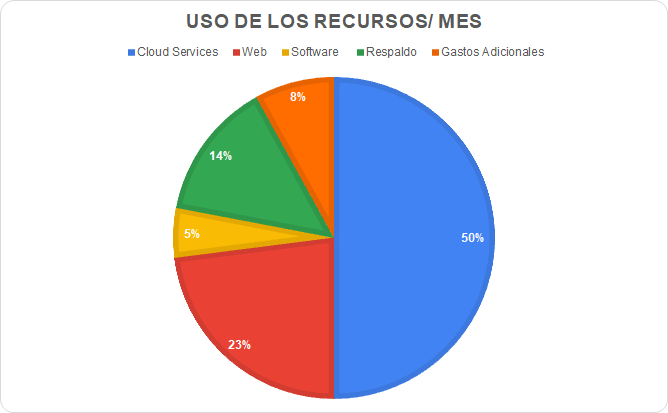
\includegraphics[width=15cm]{TC1.png}
\centering
\caption{Pie Chart sobre la Asignaci\'on de Recursos}
\end{figure}

Dentro de los recursos que se asignan a los cloud services estos se distribuyen de la siguiente forma:

\begin{table}[ht]
\centering
\begin{tabular}{|l|l|}
\hline
\multicolumn{1}{|c|}{\textbf{Recurso}} & \multicolumn{1}{c|}{\textbf{Porcentaje}} \\ \hline \hline
Almacenamiento en BigQuery             & 10                                       \\ \hline
Consultas en BigQuery                  & 5                                        \\ \hline
Seguridad                              & 85                                       \\ \hline
\end{tabular}
\caption{Desglose sobre Cloud Services}
\end{table}

\begin{figure}[ht]
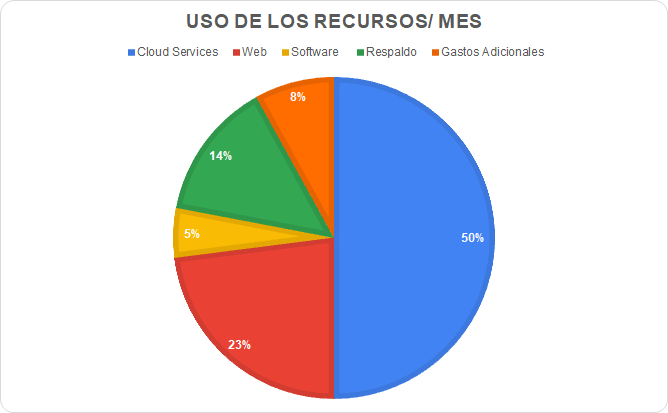
\includegraphics[width=15cm]{TC1.png}
\centering
\caption{Pie Chart sobre el Desglose de Cloud Services}
\end{figure}

\section{Anexos}
Paginas web sobre las diferentes herramientas descritas en el perfil de proyecto, como ser: paginas de documentaci\'on, informacion general y calculadoras para costos de servicios en la nube:

\begin{itemize}
    \item \url{https://grow.google/dataanalytics/#?modal_active=none}
    \item \url{https://cloud.google.com/}
    \item \url{https://www.webfx.com/website-maintenance-pricing.html}
    \item \url{https://cloud.google.com/bigquery/docs/slots}
    \item \url{https://cloud.google.com/bigquery/docs/reservations-intro}
    \item \url{https://cloud.google.com/network-connectivity/docs/vpn/pricing?hl=es-419}
    \item \url{https://cloud.google.com/bigquery/pricing}
    \item \url{https://cloud.google.com/skus/?filter=bigquery&currency=USD}
    \item \url{https://www.huaweicloud.com/intl/en-us/pricing/#/cbr}
    \item \url{https://azure.microsoft.com/en-us/pricing/calculator/}
    \item \url{https://cloud.google.com/sql/pricing#mysql-pg-pricing}
    \item \url{https://azure.microsoft.com/en-us/pricing/details/azure-sql-database/single/}
    \item \url{https://aws.amazon.com/s3/pricing/}
    \item \url{https://calculator.aws/#/createCalculator/RDSMySQL}
    \item \url{https://docs.docker.com/engine/reference/commandline/docker/}
    \item \url{https://hub.docker.com/r/jupyter/base-notebook}
    \item \url{https://www.avenga.com/our-expertise/data-services/}
    \item \url{https://www.talend.com/resources/what-is-data-as-a-service/}
    \item \url{https://help.tableau.com/current/pro/desktop/en-us/gettingstarted_overview.htm}
    \item \url{https://docs.microsoft.com/en-us/power-bi/}
    \item \url{https://docs.docker.com/}
    \item \url{https://jupyter-notebook.readthedocs.io/en/stable/}
    \item \url{https://support.huawei.com/enterprise/es/category/cloud-computing-pid-7919788}
    \item \url{https://docs.aws.amazon.com/}
    \item \url{https://docs.microsoft.com/en-us/azure/?product=featured}
\end{itemize}
















\end{document}

%%%%%%%%%%%%%%%%%%%%%%%%%%%%%%%%%%%%%%%%%%%%%%%%%%%%%%%%%%%%%%%%%%%%%%%%%%%%%%%%%%%%%%%%%%%%%%%%%%%%%%%%%%%%
%%%%%%%%%%%%%%%%%%%%%%%%%%%%%%%%%%%%%%%%%%%     FINAL     %%%%%%%%%%%%%%%%%%%%%%%%%%%%%%%%%%%%%%%%%%%%%%%%%%
%%%%%%%%%%%%%%%%%%%%%%%%%%%%%%%%%%%%%%%%%%%%%%%%%%%%%%%%%%%%%%%%%%%%%%%%%%%%%%%%%%%%%%%%%%%%%%%%%%%%%%%%%%%%